\documentclass[tikz,border=5pt]{standalone}
\usepackage{tikz}
\usepackage{xcolor}
\usetikzlibrary{calc,backgrounds}

\definecolor{bggray}{HTML}{F2F3F5}

\begin{document}
	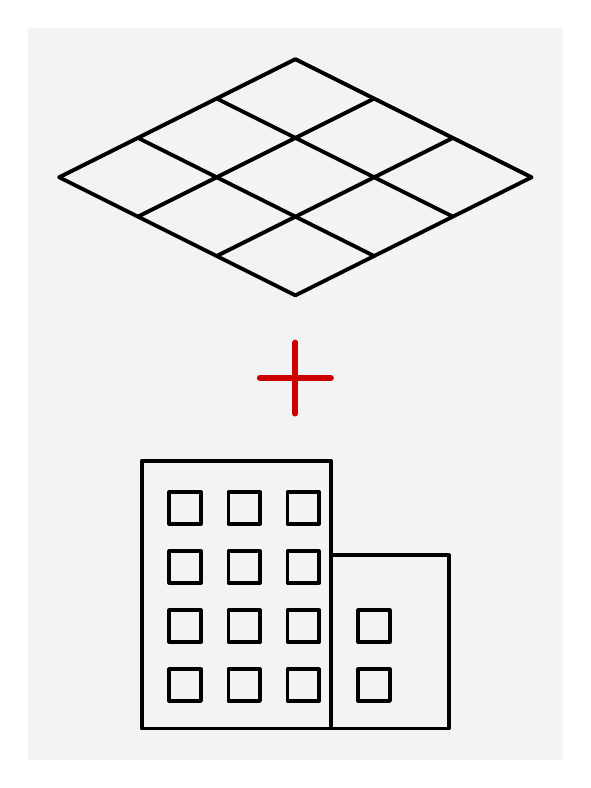
\begin{tikzpicture}[
		line width=1.4pt,
		line cap=round,
		line join=round
		]
		\fill[bggray] (-3.4,-0.4) rectangle (3.4,8.9);
		
		\begin{scope}[xshift=0cm, yshift=5.5cm]
			\coordinate (O) at (0,0);
			\foreach \i in {0,...,3} {
				\draw ($(O) + \i*(-1,0.5)$) -- ($(O) + \i*(-1,0.5) + 3*(1,0.5)$);
			}
			\foreach \j in {0,...,3} {
				\draw ($(O) + \j*(1,0.5)$) -- ($(O) + \j*(1,0.5) + 3*(-1,0.5)$);
			}
		\end{scope}
		
		\begin{scope}[xshift=0cm, yshift=4.45cm, red!80!black, line width=2.2pt]
			\draw (-0.45,0) -- (0.45,0);
			\draw (0,-0.45) -- (0,0.45);
		\end{scope}
		
		\begin{scope}[xshift=-1.95cm, yshift=0cm]
			% Tall building (left)
			\draw (0,0) rectangle (2.4,3.4);
			\foreach \r in {0,...,3} {
				\foreach \c in {0,...,2} {
					\draw ($(0.35,0.35)+(\c*0.75,\r*0.75)$) rectangle ++(0.4,0.4);
				}
			}
			\draw (2.4,0) rectangle (3.9,2.2);
			\foreach \r in {0,...,1} {
				\draw ($(2.75,0.35)+(0,\r*0.75)$) rectangle ++(0.4,0.4);
			}
		\end{scope}
		
	\end{tikzpicture}
\end{document}
